\def\mytitle{4to2 Encoder}
\def\myauthor{Putta Shreyash Chandra}
\def\mymodule{Future Wireless Communication (FWC)}
\documentclass[10pt, a4paper]{article}
\usepackage[a4paper,outer=1.5cm,inner=1.5cm,top=1.75cm,bottom=1.5cm]{geometry}
\twocolumn
\usepackage{graphicx}
\graphicspath{{./Images/}}{}
\usepackage[colorlinks,linkcolor={black},citecolor={blue!80!black},urlcolor={blue!80!black}]{hyperref}
\usepackage[parfill]{parskip}
\usepackage{lmodern}
\usepackage{tikz}
%\documentclass[tikz, border=2mm]{standalone}
\usepackage{karnaugh-map}
%\documentclass{article}
\usepackage{tabularx}

\renewcommand*\familydefault{\sfdefault}
\usepackage{watermark}
\usepackage{lipsum}
\usepackage{xcolor}
\usepackage{listings}
\usepackage{float}
\usepackage{titlesec}

\titlespacing{\subsection}{1pt}{\parskip}{3pt}
\titlespacing{\subsubsection}{0pt}{\parskip}{-\parskip}
\titlespacing{\paragraph}{0pt}{\parskip}{\parskip}
\newcommand{\figuremacro}[5]{
    \begin{figure}[#1]
        \centering
        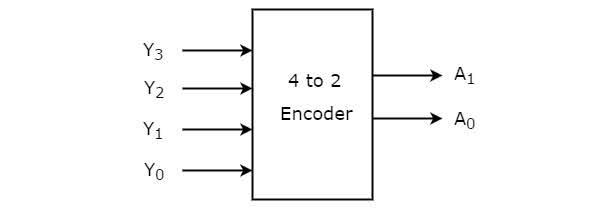
\includegraphics{Images/4_2_encoder.jpg}[width=#5\columnwidth]{#2}
        \caption[#3]{\textbf{#3}#4}
        \label{fig:#2}
    \end{figure}
}

\lstset{
frame=single, 
breaklines=true,
columns=fullflexible
}

\thiswatermark{\centering \put(400,128.0){Happy} }
\title{\mytitle}
\author{\myauthor\hspace{1em}\\IITH\hspace{0.5em}-\hspace{0.5em}\mymodule}
\date{}
\begin{document}
  \maketitle
\tableofcontents
  \begin{abstract}
      This manual shows the implementation of 4to2 encoder using Arduino ide.
     
 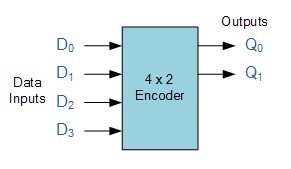
\includegraphics{Images/4_2 encoder figure with d.jpg}
    \begin{center}
     Figure 1.1  
    \end{center} 
     
 
  \end{abstract}
  \section{Components}
  \begin{tabularx}{0.4\textwidth} { 
  | >{\centering\arraybackslash}X 
  | >{\centering\arraybackslash}X 
  | >{\centering\arraybackslash}X | }
\hline
 \textbf{Components}& \textbf{Values} & \textbf{Quantity}\\
\hline
Arduino & UNO & 1 \\  
\hline
JumperWires& M-M & 7 \\ 
\hline
Breadboard &  & 1 \\

\hline
LEDs & - & 2 \\
\hline
\end{tabularx}
   \section{Implementation}
         The truth table  for Figure -1.1 is available in Table-1


  \begin{tabularx}{0.46\textwidth} { 
  | >{\centering\arraybackslash}X 
  | >{\centering\arraybackslash}X 
  | >{\centering\arraybackslash}X
  | >{\centering\arraybackslash}X 
  | >{\centering\arraybackslash}X 
  | >{\centering\arraybackslash}X |}
\hline
 D3 & D2 & D1 & D0 & Q1 & Q0 \\
\hline
0 & 0 & 0 & 1 & 0 & 0 \\  
\hline
0 & 0 & 1 & 0 & 0 & 1 \\ 
\hline
0 & 1 & 0 & 0 & 1 & 0\\
\hline
1 & 0 & 0 & 0 & 1 & 1 \\
\hline


\end{tabularx}
\begin{center}
TABLE 1.1
  \end{center}
  The Digital Encoder more commonly called a Binary Encoder takes ALL its data inputs one at a time and then converts them into a single encoded output. So we can say that a binary encoder, is a multi-input combinational logic circuit that converts the logic level “1” data at its inputs into an equivalent binary code at its output.
  
  \paragraph{Karnugh Map :}
  \paragraph{}
\textit{K-map for Q0 :}
\begin{center}

     \begin{karnaugh-map}[4][4][1][$D2D3$][$D0D1$]
        \minterms{2,8}
        \maxterms{0,1,3,4,5,6,7,9,10,11,12,13,14,15}
        \implicant{2}{2}
        \implicant{8}{8}
    \end{karnaugh-map}
    
\end{center}
{K-map for Q1 :}
\begin{center}

     \begin{karnaugh-map}[4][4][1][$D2D3$][$D0D1$]
        \minterms{5,8}
        \maxterms{0,1,2,3,4,6,7,9,10,11,12,13,14,15}
        \implicant{5}{5}
        \implicant{8}{8}  
    \end{karnaugh-map}
\end{center}
\begin{center}
Figure 2.1
\end{center}
Using Boolean logic, output Q0 Q1 in Table 1 can be expressed in terms of the inputs D0,D1,D2,D3 as 
\paragraph{}
{Q0=D3`.D2`.D1.D0` + D3.D2`.D1`.D0`                 (eq2.1)}
\paragraph{}
{Q1=D3`.D2.D1`.D0` + D3.D2`.D1`.D0`                          (eq2.2)}
 
 \paragraph{}
The expressions in (2.1) AND (2.2) can be minimized by the observing the outputs logic

Thus, after minimization  can
be expressed as
\paragraph{}
Q0=D1 + D3    by eq2.1
\paragraph{}  
Q1 = D2 + D3  by eq2.2
\hfill \break
Verify the truth table for Q0 and Q1 in TABLE 1.1.
\hfill \break

\subsection{SOLUTION :}

\paragraph{}
5,6,7,8 Pins of Arduino are manually given inputs as D1,D2,D3,D0 and verify the logic of Q0,Q1 in Table 1

\begin{tabularx}{0.60\textwidth} { 
  | >{\centering\arraybackslash}X 
  | >{\centering\arraybackslash}X 
  | >{\centering\arraybackslash}X 
  | >{\centering\arraybackslash}X 
  | >{\centering\arraybackslash}X 
  | >{\centering\arraybackslash}X
  | >{\centering\arraybackslash}X
  | >{\centering\arraybackslash}X|}

\hline
 \textbf{Encoder} & D1 & D2 & D3 & D0 & Q1 & Q0 \\
\hline
\textbf{Arduino} & 5 & 6 & 7 & 8 & 13 & 4 \\  
\hline
\end{tabularx}
 
\begin{center}
TABLE 2.1
\end{center}

The code below realizes the Boolean logic for 4to2 encoder in 1.1  using 5V,GND of Arduino as binary Inputs with the help of breadboard and jumperwires.
Built in LED at pin-13 of Arduino will glow for the logic'1' of Q1,and off for the logic'0' of Q1  and a LED circuit at pin-4 of Arduino will glow for the logic'1' of Q0,and off for the logic'0' of Q0
\begin{lstlisting}
https://github.com/chanduputta/FWC-Module1/blob/main/IDE%20assignment/code/main.cpp
\end{lstlisting}
\bibliographystyle{ieeetr}
\end{document}
